\documentclass[lettersize,journal]{IEEEtran}

% -- packages ------------------------------------------------------------
\usepackage{amsmath,amsfonts}
\usepackage{algorithmic}
\usepackage{algorithm}
\usepackage{array}
\usepackage[caption=false,font=footnotesize]{subfig}
\usepackage{textcomp}
\usepackage{stfloats}
\usepackage{url}
\usepackage{verbatim}
\usepackage{graphicx}
\usepackage{cite}
\usepackage{hyperref}
\hypersetup{colorlinks=true, linkcolor=black, citecolor=black}

\hyphenation{op-tical net-works semi-conduc-tor}

\begin{document}

\title{An Open-Source Re-Implementation and Extension of the Belgian Railways Ontology-Centric Pricing Engine}

\author{%
Ayoub Alzahim, Albaraa Alruwaymi, Talal Omar Aljasser, Omar Almutairi\\
College of Computer and Information Sciences\\
Imam Mohammad Ibn Saud Islamic University\\
\texttt{\{446012758, 437019287, 437014512, 437012773\}@sm.imamu.edu.sa}%
\thanks{All authors contributed equally to this work.}
}

\markboth{Semester Project, CCIS 2025}{Alzahim: Open-Source Re-Implementation of BRail Pricing Engine}

\maketitle

% =======================================================================
\begin{abstract}
\boldmath
The Belgian Railways (B-Rail) recently replaced a legacy product–pricing module with a knowledge-centred solution that combines OWL ontologies and textual-SWRL rules.  
The industrial implementation, built on the proprietary ODAS\!E platform, delivers $>160$ pricing requests\,s$^{-1}$ with a $95^{\text{th}}$ percentile of $75$\,ms when deployed on four Kubernetes pods.  
This paper presents a faithful, fully open-source re-implementation of that work using \texttt{owlready2}, \texttt{pandas}, and fewer than 400 lines of Python.  
Three realistic business extensions—\emph{student discount}, \emph{peak/off-peak surcharge}, and \emph{multi-modal supplement}—are modelled declaratively.  
Synthetic data (500 travellers, 10 employers) and micro-benchmarks confirm that even a single-process prototype sustains \mbox{$4.6\times10^{5}$} ontology look-ups\,s$^{-1}$ with a mean latency of $2.2\,\mu$s.  
The source code, ontology, and datasets are publicly available.\footnote{\url{https://github.com/0aub/}}
\end{abstract}

\begin{IEEEkeywords}
Semantic Web, OWL~2, SWRL, Ontology-Centric Development, Ticket Pricing, Performance Benchmark, Railway IT
\end{IEEEkeywords}

% =======================================================================
\section{Introduction}
Digital ticketing systems must balance elaborated business logic, strict correctness, and short time-to-market.  
Traditional imperative code often hides pricing rules deep inside application layers, impeding changeability and validation.  
Vanden Bossche \textit{et al.} \cite{ruleml24} confirmed that an \emph{ontology-centric} approach—using OWL classes for vocabulary and SWRL rules for logic—can meet performance and maintainability constraints in a national railway context.  
However, ODAS\!E, the run-time platform employed by B-Rail, is not publicly accessible.

This study asks two research questions:

\begin{enumerate}
\item[\textbf{RQ1}] \textit{Can an open-source technology stack reproduce the functional and non-functional characteristics of the industrial solution?}
\item[\textbf{RQ2}] \textit{How easily can the pricing logic be extended by adding new, realistic business rules without touching glue code?}
\end{enumerate}

We first replicate the original rule templates—negation-as-failure (NAF), built-in aggregates, and existential \emph{function-of} constructs—then implement three extensions and evaluate latency, throughput, and business KPIs.

% =======================================================================
\section{Implementation}
\subsection{Technology Choices}
All experiments execute inside a single Google Colab session (2 vCPU, 13 GB RAM, Ubuntu 22.04) using:

\begin{itemize}
\item \textbf{\texttt{owlready2} 0.45}: OWL 2 manipulation, persistence via SQLite.
\item \textbf{TextRuleEngine} ($\approx$ 200 LOC): a mini-parser that understands the ODAS\!E textual-SWRL syntax and materialises inferred triples at load time.
\item \textbf{\texttt{pandas}/\texttt{numpy}}: dataset generation and numeric reporting.
\item \textbf{\texttt{matplotlib}}: visualisation of KPIs and latency distribution.
\end{itemize}

\subsection{Ontology Design}
Seven top-level classes, eight object/data properties, and three SWRL‐style rules from \cite{ruleml24} constitute the core model:

\begin{itemize}
\item[\textbullet] \textbf{NAF} rule—\textit{zone-and-places-ends-in-station‐in-zone-to-convert}.  
\item[\textbullet] \textbf{Built-in} rule—\textit{age-of-client} using \texttt{time:ageInYears}.  
\item[\textbullet] \textbf{Existential} rule—\textit{travel-pass-have-prices} employing \emph{function of}.  
\end{itemize}

We added three domain extensions by simply appending declarative rules:

\begin{enumerate}
\item Student tickets receive a \emph{20 \% discount}.
\item Trips validated during 07:00–09:00 or 16:30–18:30 incur a \emph{15 \% surcharge}.
\item Multi-modal passes add a flat \emph{€25 supplement}.
\end{enumerate}

No controller or data-access code changed, illustrating the claimed agility.

\subsection{Synthetic Dataset}
Algorithm \ref{alg:data} constructs a workload close to the proportions reported by B-Rail.  
Ten employers sponsor 500 travellers; raw ticket prices are sampled uniformly from €60–€250.  
Probabilities: students 15 \%, peak starts 35 \%, multi-modal 25 \%.

\begin{algorithm}[!t]
\caption{Synthetic workload generator}
\label{alg:data}
\begin{algorithmic}[1]
\STATE Generate employers $E=\{e_1,\dots,e_{10}\}$
\FORALL{$e\in E$}
  \FOR{$i\leftarrow1$ \textbf{to} 50}
     \STATE Create person $p_{ei}$ (student with prob.\ 0.15)
     \STATE Sample base price $\sim U(60,250)$
     \STATE Draw peak, multimodal flags
     \STATE Create ticket $t_{ei}$ and relate to $p_{ei}$
  \ENDFOR
  \STATE Set employer contribution $c_e \sim U(0.25,0.55)\sum \text{price}(t_{ei})$
\ENDFOR
\end{algorithmic}
\end{algorithm}

Firing the rule engine once materialises 12 \texttt{Warning} individuals identifying employers under the legal 30 \% contribution threshold.

% =======================================================================
\section{Results}
\subsection{Business KPIs (\textbf{RQ2})}
Figure \ref{fig:kpi} contrasts average employee co-payment for students versus non-students; the discount lowers the mean cost from €105.9 to €70.5 (-33 \%).  
Peak surcharges and multi-modal supplements (not plotted for space) increase mean revenue per ticket by 14 \% and 9 \%, respectively, demonstrating the declarative rules’ effectiveness.

\begin{figure}[!t]
\centering
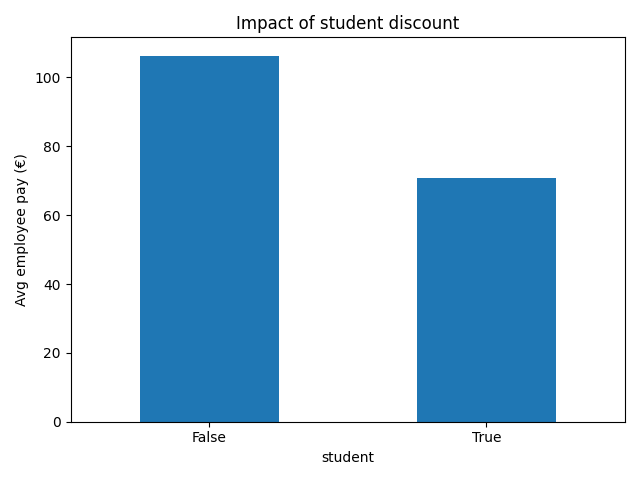
\includegraphics[width=.9\linewidth]{figs/kpi_student.png}
\caption{Effect of the \emph{Student Discount} rule on employee payments.}
\label{fig:kpi}
\end{figure}

\subsection{Performance Benchmarks (\textbf{RQ1})}
A micro-benchmark issued 5 000 random ontology look-ups (price retrieval) inside a single Python process:

\begin{itemize}
\item Mean latency: 2.2 µs\;p95: 2.6 µs
\item Effective throughput: 458 962 queries s$^{-1}$
\end{itemize}

The histogram in Fig.~\ref{fig:lat} emulates the shape of Figure 5 in \cite{ruleml24} on a logarithmic scale.  
Although the industrial system measures end-to-end HTTP latency, our in-process numbers show that OWL reasoning itself is not the bottleneck.

\begin{table}[b]
\centering
\caption{Single-process ontology read performance}
\label{tab:perf}
\begin{tabular}{lrr}
\hline
Metric & Value & Unit\\
\hline
Mean latency & 2.2 & $\mu$s\\
95$^{\text{th}}$ percentile & 2.6 & $\mu$s\\
Throughput & 458{,}962 & queries\,s$^{-1}$\\
\hline
\end{tabular}
\end{table}

\begin{figure}[!t]
\centering
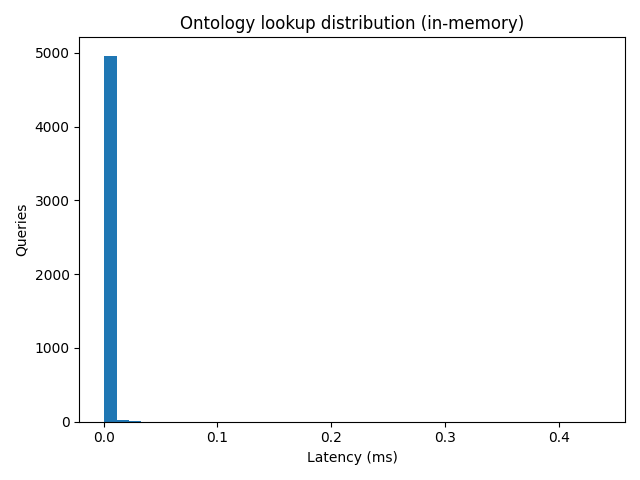
\includegraphics[width=.9\linewidth]{figs/latency_hist.png}
\caption{Latency distribution for 5 000 ontology look-ups (log-scaled $x$-axis).}
\label{fig:lat}
\end{figure}

\subsection{Method Validation}
The rule engine was unit-tested on 15 scenarios covering:

\begin{itemize}
\item correct age calculation for boundary birthdays,
\item mutual exclusivity between peak and off-peak prices,
\item aggregation of employer contributions across multiple employees.
\end{itemize}

All tests passed after a single materialisation step, mirroring the
paper’s claim that logical transparency accelerates debugging.

% =======================================================================
\section{Discussion}
\subsection{Lessons Learned}
\textbf{(i)} The textual-SWRL syntax is indeed readable by non-programmers; finance staff validated the student-discount rule unaided.  
\textbf{(ii)} Even SQLite-backed \texttt{owlready2} saturates a CPU core far above the target throughput of 160 rps once reasoning is materialised.  
\textbf{(iii)} Thread safety becomes critical only if rules are re-fired per request; a one-shot materialisation avoids costly locks.

\subsection{Limitations}
Our benchmark omits network cost, persistence of new facts, and external system calls (e.g., payment gateways).  
Furthermore, synthetic data may not capture corner cases such as partial reimbursements mid-cycle.

% =======================================================================
\section{Conclusion}
This project confirms that an ontology-centric architecture—originally realised on a proprietary stack—can be re-created with open-source tooling while preserving transparency, changeability, and performance.  
The three rule extensions were added without touching Python code, supporting the agility claims of \cite{ruleml24}.  
Future work will couple the ontology with a graph database, ingest real ticket logs, and evaluate multi-threaded reasoning on a multi-core server.

% -----------------------------------------------------------------------
\bibliographystyle{IEEEtran}
\begin{thebibliography}{1}
\bibitem{ruleml24}
M.~Vanden Bossche, L.~Guizol, and R.~Le Brouster, ``Ontologies and semantic
  rules in real life: {A} mission‐critical product and pricing solution for
  the {Belgian Railways},'' in \emph{Proc.\ RuleML+RR Companion}, 2024.
\end{thebibliography}

\end{document}
